\section{Compact ODD-style Model Summary}
\label{sec:appendix-odd}

\textbf{Purpose.} Generate, from elementary micro-level social,
ecological, and organizational rules, whatever persistent macro-level
institutional patterns emerge, without encoding or optimizing toward any
predefined governance typology.

\textbf{Entities, state variables, scales.} Heterogeneous agents
(resources, relational memory, behavioral and ecological policies,
proposal/membership/enforcement traits, migration propensity); a dynamic
relationship network; a fixed number of resource patches, each with a
carrying capacity and logistic regeneration; shared rules
(\texttt{SharedRule}) with a 14-slot component bundle and full lineage
provenance (\texttt{InstitutionRecord}); delegates with realized-
performance-based administrative capacity; bilateral coordination links
between patches. Population 32--80, patches 3--6, runs up to 700 steps
across the reported experiments.

\textbf{Process overview and scheduling.} Each step: perturbations (if
scheduled); bilateral social interactions; ecological actions
(extraction/maintenance/restraint) and subsistence; patch regeneration;
memory decay; relationship dynamics (periodic); social and ecological
adaptation (periodic); institution lifecycle bookkeeping; local
institutional observation; component-wise transmission; migration and
membership exit; delegation (accountability, nomination/selection, task
performance); coordination (proposal/acceptance/activity/dissolution);
institutional scaling; observer metrics computed from a read-only
snapshot.

\textbf{Design concepts.} Bottom-up emergence with no global planner or
designed target state; strict generative/observer separation, enforced by
an abstract-syntax-tree-based import-direction test; every mechanism
introduced after Level 0 defaults to a verified, byte-for-byte no-op;
every stochastic draw passes through one explicit, seeded random-number
generator per run (or, for causal experiments, a per-mechanism substream
architecture).

\textbf{Initialization.} Agent traits and patch memberships are drawn once
at build time from configured distributions; no institution exists at
initialization unless a run explicitly injects one as an initial-condition
family (Level 1.2b's heterogeneous proto-institution family).

\textbf{Input data.} None. No external empirical dataset, including the
companion dissertation's own survey data, is ever read by any generative,
observer, or experiment-script code; mechanically audited by a dedicated
firewall test in both milestones.

\textbf{Submodels.} See \cref{sec:model-methods} and the source
repository's own \texttt{docs/odd\_level0.1.md} through
\texttt{docs/odd\_level1.3\_addendum.md} for full per-mechanism
specifications.

\textbf{Level 1.3/1.3b ODD addendum (compact).} \textit{State variables
added:} accumulated pressure history per channel (security, bargaining,
coordination-complexity), institutional entrenchment (age-dependent
amendment/dissolution resistance), and two independent legitimacy ledgers
(performance, procedural), all agent/institution-level and read by the
generative layer; observer-only $S_{\text{obs}}$/$Z_{\text{obs}}$
composites, read-only, never fed back. \textit{Process overview addition:}
each step, if a pressure channel is active, its current level is computed
and applied via one or two of six shared transmission primitives
(\texttt{pressure\_adjusted\_probability}, \texttt{pressure\_adjusted\_%
scale}) to the specific decision or quantity that channel targets;
entrenchment accumulates with institution age and is consulted wherever an
amendment or dissolution decision already occurs; legitimacy ledgers
accumulate from realized outcomes/procedure and decay per existing
legitimacy dynamics, now split into two independently tracked series.
\textit{Design concepts added:} every historical mechanism defaults to a
verified no-op, confirmed behavior-identical to Level 1.2b at every
disabled setting; Level 1.3b's own checkpoint/fork machinery
(\texttt{core/state\_checkpoint.py}) supports mid-run branching for causal
intervention experiments, sham-validated against spurious divergence.
\textit{Initialization:} unchanged from Level 1.2b; historical state
variables begin at zero/inactive unless a stage script explicitly seeds
pressure history for a causal-intervention arm. \textit{Input data:} none,
as at every prior milestone; the SEM firewall (\cref{sec:appendix-software})
extends unmodified to every Level 1.3/1.3b module and document.

\clearpage
\section{Parameter Tables}
\label{sec:appendix-parameters}
\label{sec:appendix-tables}

\begin{table}[htbp]
\centering
\caption{Selected configuration parameters relevant to Level 1.2/1.2b
results (full reference: source repository \texttt{docs/config\_%
reference.md}).}
\label{tab:parameters}
\begin{tabular}{@{}p{0.27\textwidth}p{0.36\textwidth}p{0.30\textwidth}@{}}
\toprule
\textbf{Parameter} & \textbf{Default} & \textbf{Role} \\
\midrule
\texttt{population\_size} & 60 (Level 0); 32--80 (L1.2/1.2b runs) & Agent count \\
\texttt{n\_patches} & 4 (typ.); 3--6 in scaling grids & Independent resource patches \\
\texttt{patch\_capacity} & 500.0 & Per-patch carrying capacity $K_j$ \\
\texttt{patch\_regen\_rate} & 0.5 (default); 0.2--1.0 swept & Logistic regeneration rate $r_j$ \\
\texttt{patch\_initial\_fraction} & 0.5 & Initial stock as fraction of $K_j$ \\
\texttt{subsistence\_cost} & config-dependent; 0.1--0.6 swept (WP N) & Mandatory per-agent per-step cost \\
\texttt{ecological\_harvest\_unit} & 5.0 & Extraction-propensity $\to$ resource-unit scale \\
\texttt{ecological\_maintenance\_unit} & 5.0 & Maintenance-investment $\to$ resource-unit scale \\
\texttt{maintenance\_efficiency} & 0.7 (default); 0.3--1.0 swept & Fraction of investment reaching the patch \\
\texttt{migration\_enabled} & False (default) & Gate for agent relocation \\
\texttt{migration\_capacity\_per\_patch} & config-dependent; 0.05--0.4 swept (rate), 0--4 (cost) & Migration mechanics \\
\texttt{institutional\_transmission\_enabled} & False (default) & Gate for component-wise transmission \\
\texttt{transmission\_base\_probability} & config-dependent; cost 0.01--0.2 swept & Per-attempt transmission probability \\
\texttt{delegation\_enabled} & False (default) & Gate for delegation/administration \\
\texttt{discretion\_enabled} & False (default) & Gate for appropriation/effort-withholding \\
\texttt{accountability\_enabled} & False (default) & Gate for audit/recall/appeal \\
\texttt{interpatch\_coordination\_enabled} & False (default) & Gate for bilateral coordination links \\
\texttt{coordination\_cost\_per\_step} & config-dependent; 0.0--0.2 swept & Per-step per-link maintenance fee \\
\texttt{scaling\_admin\_overhead\_per\_patch} & config-dependent; 0.0--0.2 swept & Jurisdiction-scale admin overhead \\
\texttt{rng\_mode} & \texttt{"legacy\_single\_stream"} (default); \texttt{"mechanism\_substreams"} (mandatory for causal runs) & RNG discipline \\
\texttt{n\_steps} & 500 (Level 0); 350--700 by stage & Run duration \\
\bottomrule
\end{tabular}


\medskip
\noindent\footnotesize Full field-level documentation:
\texttt{docs/config\_reference.md} in the source model repository. Every
row above is a no-op at its listed default unless a stage/Work Package
script explicitly overrides it, per \cref{tab:mechanism-layer}.
\normalsize
\end{table}

\clearpage
\section{Complete Outcome-Count Tables}
\label{sec:appendix-outcomes}

\Cref{tab:outcome-distribution} in the main text reports the pooled
all-outcome distribution for every major run set. This appendix adds the
two breakdowns not shown in the main text: Level 1.2b's failure-trajectory
classification (a finer-grained view of \textit{how} collapse was reached,
not merely whether it was), and the scaling-robustness grid's own
per-condition detail.

\begin{table}[htbp]
\centering
\caption{Failure-trajectory classification, discovery ($n$=576) versus
confirmation ($n$=384) pools.}
\label{tab:failure-trajectory}
\begin{tabular}{@{}lrr@{}}
\toprule
\textbf{Label} & \textbf{Discovery (WP J)} & \textbf{Confirmation (WP L)} \\
\midrule
no\_collapse\_observed              & 194 & 99 \\
transient\_dip\_recovered           & 56  & 40 \\
collapse\_onset\_after\_last\_snapshot & 0 & 0 \\
late\_onset\_collapse               & 21  & 14 \\
sustained\_collapse                 & 305 & 231 \\
\midrule
\textbf{Total} & \textbf{576} & \textbf{384} \\
\bottomrule
\end{tabular}
\end{table}

\begin{table}[htbp]
\centering
\caption{Level 1.2 Stage 6 scaling-robustness grid, per-condition detail
(2 seeds/condition, 300 steps).}
\label{tab:stage6-detail}
\begin{tabular}{@{}rrrl@{}}
\toprule
\textbf{Population} & \textbf{Patches} & \textbf{Outcome (both seeds)} & \textbf{Ecological fraction (seed 1, seed 2)} \\
\midrule
40 & 3 & collapse, collapse & 0.029, 0.013 \\
40 & 6 & collapse, collapse & 0.011, 0.024 \\
80 & 3 & collapse, collapse & 0.044, 0.025 \\
80 & 6 & collapse, collapse & 0.032, 0.019 \\
\bottomrule
\end{tabular}
\end{table}

\clearpage
\section{Recurrence Criteria}
\label{sec:appendix-recurrence-criteria}

The twelve minimum recurrence criteria, evaluated unconditionally (no
short-circuiting) and combined by strict conjunction:
\texttt{minimum\_cluster\_size}, \texttt{cross\_seed\_recurrence},
\texttt{cross\_algorithm\_support}, \texttt{bootstrap\_stability},
\texttt{co\_assignment\_internal\_consistency}, \texttt{distinctness\_%
from\_noise}, \texttt{missingness\_strategy\_robustness},
\texttt{parameter\_condition\_diversity}, \texttt{temporal\_persistence\_%
of\_members}, \texttt{non\_degenerate\_cluster\_fraction},
\texttt{k\_selection\_non\_privileged\_support},
\texttt{independent\_of\_single\_lineage}. None references cluster count
or identity. Two criterion pairs superficially resemble each other but
were confirmed, on audit, to measure genuinely distinct things and were
therefore neither merged nor dropped: \texttt{cross\_seed\_recurrence}
versus \texttt{parameter\_condition\_diversity} (seed identity and
parameter condition are different axes of variation), and
\texttt{minimum\_cluster\_size} versus \texttt{non\_degenerate\_cluster\_%
fraction} (a raw floor versus a pool-size-relative bound).

\clearpage
\section{Clustering and Confirmation Procedures}
\label{sec:appendix-clustering-procedures}

Discovery-verdict vocabulary (closed, six labels, first-match-wins):
\texttt{insufficient\_evidence} (sample size or headline $k$ undefined);
\texttt{failure\_dominated} (clustering re-derives the failure/success
split, adjusted Rand index $\geq0.5$ against a cheap proxy);
\texttt{unstable} (neither bootstrap nor algorithm-agreement adjusted Rand
index clears 0.3); \texttt{one\_config} (no $k\geq2$ clears a 0.15
silhouette floor); \texttt{continuum} (three or more evaluated $k$'s sit
within 0.05 silhouette of the best); \texttt{multi\_config} (a single,
clearly dominant silhouette peak). Confirmation-verdict vocabulary (closed,
three labels): \texttt{insufficient\_confirmation\_data},
\texttt{null\_replicated}, \texttt{unexpected\_recurring\_structure}. The
null-replication rule: if discovery supports no discrete candidates
--- including a \texttt{continuum} verdict --- confirmation replicates the
null result on fresh data rather than manufacturing a candidate to test.

Level 1.3b's own extended discovery-verdict vocabulary (closed, eight
labels, applied specifically to the historical-effect question): \texttt{A%
\_no\_effect}; \texttt{B\_pressure\_responsive\_nonhistorical} (responds to
pressure magnitude, not order/history); \texttt{C\_transient}
(differentiation reconverges); \texttt{D\_persistent\_continuum}
(persistent path dependence, continuous gradient); \texttt{E\_two\_%
families}; \texttt{F\_three\_families}; \texttt{G\_four\_or\_more\_%
families}; \texttt{H\_inconclusive}. \texttt{DECISION\_GATE\_DO\_NOT\_%
PREFER = "F\_three\_families"} scopes explicitly to mean only that the
discovery pipeline's own default must not be biased toward three families,
not that F is disqualified as a genuine finding if the evidence actually
supports it; no Level 1.3b script special-cased or biased toward F, and
F was ruled out on the same evidence that ruled out E and G, not singled
out for extra scrutiny. Ruling out E/F/G reuses Level 1.2b's own frozen
\texttt{classify\_discovery\_verdict} unmodified, applied to Level 1.3b's
own Stage 7 leading discrete candidate.

\clearpage
\section{Accounting Identities}
\label{sec:appendix-accounting}

The ecological ledger reconciles, for an arbitrary window
$[t_0, t_1)$:
\[
\text{opening stock} + \text{total supply} - \text{total demand} = \text{closing stock}
\]
computed from the event log plus a patch-system snapshot at each end of
the window, where \textbf{supply} = patch regeneration + appeal refunds +
recall-recovered funds; \textbf{demand} = ecological extraction +
maintenance investment + subsistence + administrative cost + appropriation
+ contribution/fund-dissolution loss + shock loss (patches topology) +
monitoring cost + sanction cost/penalty + bilateral punishment cost/
penalty + relationship-exit cost + relationship-formation search cost +
audit cost + voluntary membership-exit cost + per-active-link coordination
maintenance fee; and interpatch migration and mutual-assistance transfers
are net-zero (resources move with the transaction, no system-level gain or
loss). Post-fix, production-scale residual: $\sim10^{-10}$ per seed
(maximum $5.9\times10^{-9}$ across the full 576-run discovery design,
against a documented tolerance of $10^{-4}$).

\clearpage
\section{Experiment / Run-Count Table}
\label{sec:appendix-run-counts}

See \cref{tab:run-counts} in the main text for the complete run-count
table by component; it is not repeated here.

\clearpage
\section{Disclosed Scope Reductions}
\label{sec:appendix-scope-reductions}

\begin{table}[htbp]
\centering
\caption{Every disclosed scope reduction carried by Level 1.2 or Level
1.2b, recorded before the affected component ran.}
\label{tab:scope-reductions}
\adjustbox{max width=\textwidth}{\begin{tabular}{@{}lp{0.75\textwidth}@{}}
\toprule
\textbf{Component} & \textbf{Disclosed reduction} \\
\midrule
L1.2 discovery pipeline & 3 candidate clustering methods (of a fuller suggested menu); $k=1$--8 only. \\
L1.2 Stage 1 & 8 seeds/condition, population 40, 350 steps. \\
L1.2 Stage 2 & 10 seeds, population 40, 400 steps. \\
L1.2 Stage 3 & 12 parameter draws $\times$ 2 seeds = 24 total runs (of a larger publication-scale sweep). \\
L1.2 Stage 5 & 12 fresh runs (reusing Stage 3's own 12 parameter draws, fresh seeds). \\
L1.2 Stage 6 & 4 scale conditions $\times$ 2 seeds = 8 total. \\
L1.2 Stage 7 & 2 perturbation types $\times$ 3 seeds = 6 shocked/unshocked pairs. \\
L1.2 Section 13 & 2 ablations $\times$ 8 matched-seed pairs each. \\
L1.2b Work Package G & 4 burn-in-sensitivity definitions validated on a 12-seed-run subset (3 points $\times$ 2 seeds $\times$ 2 IC families) of the full 576-run pool. \\
L1.2b Work Package O & \texttt{shared\_lineage\_persistence} not evaluated (would require a 4th 576-run re-simulation with per-run lineage export); disclosed as an evidence gap, not filled. \\
\bottomrule
\end{tabular}
}

\medskip
\noindent\footnotesize Every reduction above was recorded in its own script's
docstring or output before that component ran, never adjusted afterward to
match results (Level 1.2 Section 20 / Level 1.2b Section 27's own stop-
condition discipline).
\normalsize
\end{table}

\clearpage
\section{Software and Testing Information}
\label{sec:appendix-software}

Python-based simulation and analysis stack (\texttt{numpy}, and standard
scientific-Python clustering/statistics utilities for Gaussian mixtures,
hierarchical clustering, \texttt{HDBSCAN}, silhouette/Calinski--Harabasz/
Davies--Bouldin metrics, and the adjusted Rand index); \texttt{pytest} for
the test suite. Test-suite status: 1,084 passed / 6 skipped / 0 failed / 0
warnings at the close of Level 1.2 (\texttt{python -m pytest -q -W
error}); 1,475 passed / 6 skipped / 0 failed / 0 warnings at the close of
Level 1.2b (389 new tests); 1,869 passed / 6 skipped / 0 failed / 0
warnings at the close of Level 1.3 (Level 1.3b's own disclosed preflight
baseline); and 2,047 passed / 6 skipped / 0 failed / 0 warnings at the
close of Level 1.3b (178 new tests across 19 files, exactly matching the
delta from the 1,869 baseline). A whole-package forbidden-terminology
structural guard and a dedicated SEM-firewall audit (confirming no
dissertation-derived data file exists anywhere in the repository) both
passed throughout all four milestones; Level 1.3b's own extension adds a
docs-directory scan for \texttt{docs/level1.3b\_*.md} and reuses Level
1.3's own forbidden-term list unmodified.

This paper's own \LaTeX{} build: \texttt{pdflatex} + \texttt{biber},
orchestrated by \texttt{latexmk} (fallback: manual \texttt{pdflatex}/
\texttt{biber}/\texttt{pdflatex}/\texttt{pdflatex} sequence, see
\texttt{Makefile}); TeX Live 2023 (Debian).

\clearpage
\section{Evidence Ledger (Condensed)}
\label{sec:appendix-ledger}

The complete evidence ledger, mapping every numerical claim in this paper
to its exact source file and field in the source model repository's own
output artifacts, is maintained at \texttt{dev\_mem/evidence\_ledger.md}
(Level 1.2/1.2b claims) and \texttt{claim\_evidence\_manifest.csv} at this
repository's root (every Level 1.3/1.3b and dissertation-sourced claim,
with design type, denominator, uncertainty, and disclosed limitations as
separate columns, per this revision's own reporting requirements). Each
record includes the claimed value, the exact source file, the exact field
or computation used to derive it, and a verification status (recomputed
directly from raw JSON output; taken from a cross-checked prose document;
or an explicitly disclosed gap). No discrepancy was found between any
prose summary in the source repository and its own underlying raw output
during this paper's preflight, for either the original Level 1.2/1.2b
audit or this revision's own Level 1.3/1.3b audit. Selected headline
entries (Level 1.2/1.2b; see \texttt{claim\_evidence\_manifest.csv} for the
Level 1.3/1.3b equivalents):

\begingroup
\raggedright
\begin{itemize}
\item Level 1.2 Stage 3: 22/24 collapse --- \texttt{outputs/level12\_%
stage3\_main\_search/stage3\_report.json}, field \texttt{outcome\_label\_%
distribution}.
\item Level 1.2 Stage 4/5: 0/76 and 0/72 candidates meeting all 12
criteria --- \texttt{outputs/level12\_stage4\_blind\_discovery/}\allowbreak%
\texttt{stage4\_report.json} and \texttt{outputs/level12\_stage5\_prospective\_%
confirmation/}\allowbreak\texttt{stage5\_report.json}.
\item Level 1.2b ledger residual $\sim10^{-10}$, pre-fix 9.14 ---
\texttt{docs/level1.2b\_ecological\_accounting.md} \S2.
\item Level 1.2b feasibility-ratio correlations $r\approx0.84$/$0.48$ ---
\texttt{outputs/level12b\_stage\_c\_feasibility\_map/results.json}, field
\texttt{ex\_ante\_vs\_realized\_correlation}.
\item Level 1.2b discovery/confirmation outcome distributions (326/161/89;
245/86/53) --- \texttt{outputs/level12b\_stage\_j\_main\_discovery\_%
pipeline/}\allowbreak\texttt{results.json} and \texttt{outputs/level12b\_stage\_l3\_%
prospective\_confirmation/}\allowbreak\texttt{results.json}, field \texttt{all\_outcome\_%
summary}.
\item Level 1.2b scaling-robustness outcome distribution (25/4/3) and
recovery rates (0\%/87.5\%) --- \texttt{outputs/level12b\_stage\_m\_%
scaling\_robustness/results.json}, recomputed directly from per-run
records (\texttt{transition\_to\_failure.all\_outcome\_label},
\texttt{functional\_recovery.\{population,}\allowbreak\texttt{ecological\}.recovered}).
\item Level 1.2b causal decomposition effect sizes ---
\texttt{outputs/level12b\_stage\_n\_causal\_collapse\_decomposition/}\allowbreak%
\texttt{results.json}, recomputed directly from \texttt{factor\_results[*].pairs}.
\end{itemize}
\endgroup

\clearpage
\section{Additional Figures}
\label{sec:appendix-figures}

\begin{figure}[htbp]
\centering
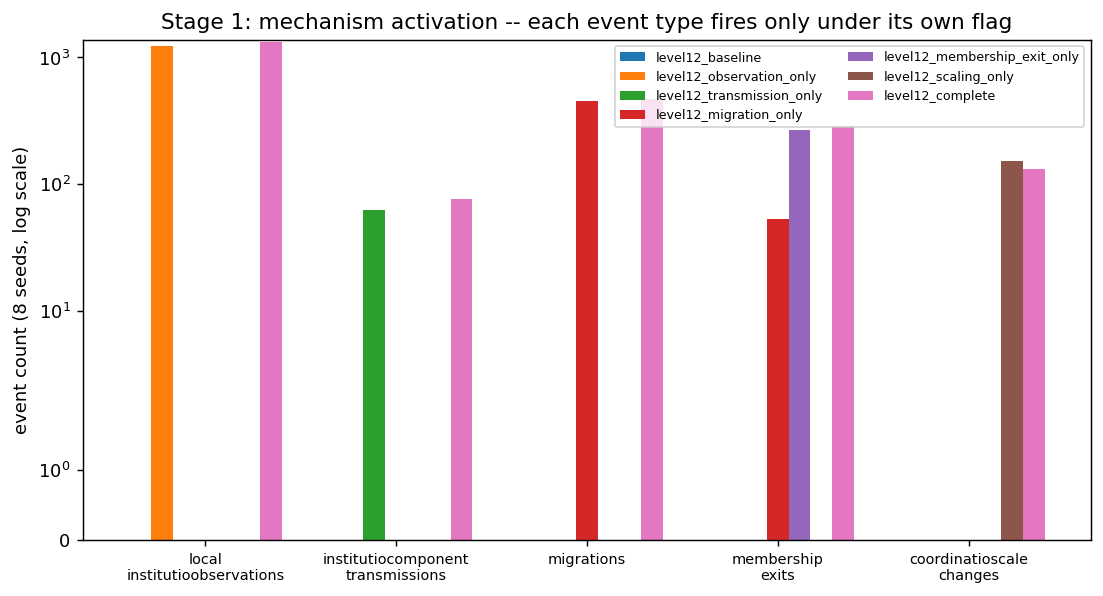
\includegraphics[width=0.75\textwidth]{figures/appendix/a_l12_stage1_activation.png}
\caption{Level 1.2 Stage 1: mechanism-activation totals across 7
conditions $\times$ 8 seeds (56 runs), confirming every new mechanism is
reachable and behaves as expected before any search stage runs.}
\end{figure}

\begin{figure}[htbp]
\centering
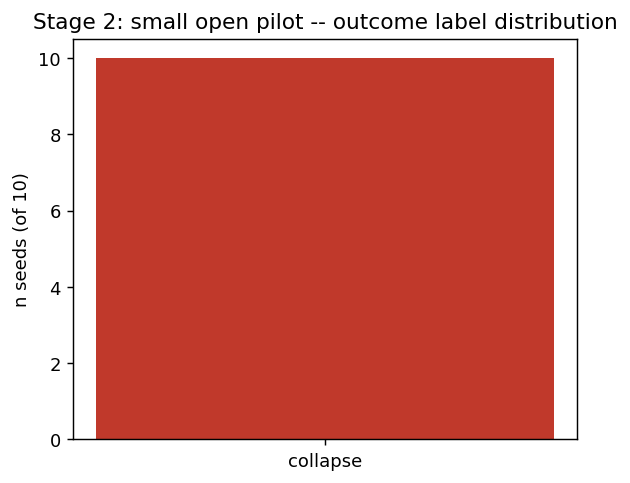
\includegraphics[width=0.7\textwidth]{figures/appendix/a_l12_stage2_outcome.png}
\caption{Level 1.2 Stage 2 small open pilot outcome distribution
($n$=10): 7 collapse, 3 fragmented, 0 viable.}
\end{figure}

\begin{figure}[htbp]
\centering
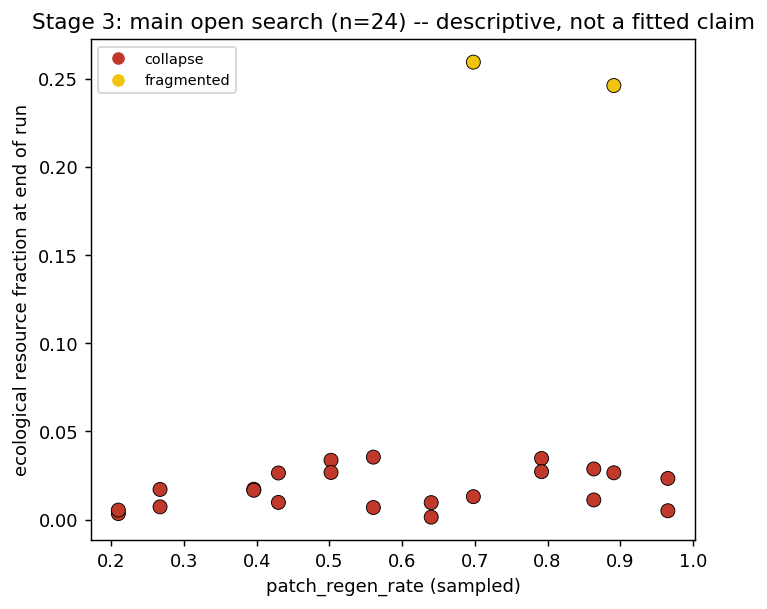
\includegraphics[width=0.75\textwidth]{figures/appendix/a_l12_stage3_regen_vs_eco.png}
\caption{Level 1.2 Stage 3: patch regeneration rate versus realized
ecological fraction across the 24-run main search --- the descriptive
association Section 13's regen-rate ablation later tested causally.}
\end{figure}

\begin{figure}[htbp]
\centering
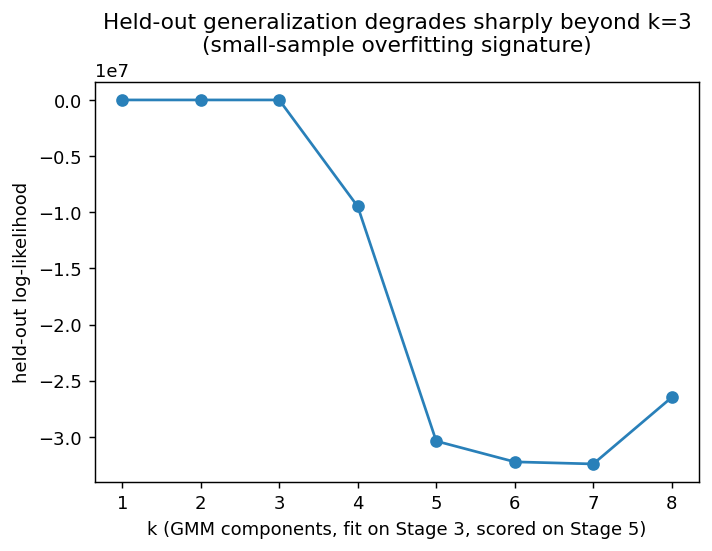
\includegraphics[width=0.7\textwidth]{figures/appendix/a_l12_stage5_heldout_ll.png}
\caption{Level 1.2 Stage 5: held-out log-likelihood by $k$, fit on Stage 3
and scored on Stage 5's fresh runs --- gradual degradation to $k$=3, then
catastrophic collapse at $k\geq4$, a small-sample Gaussian-mixture
overfitting signature.}
\end{figure}

\begin{figure}[htbp]
\centering
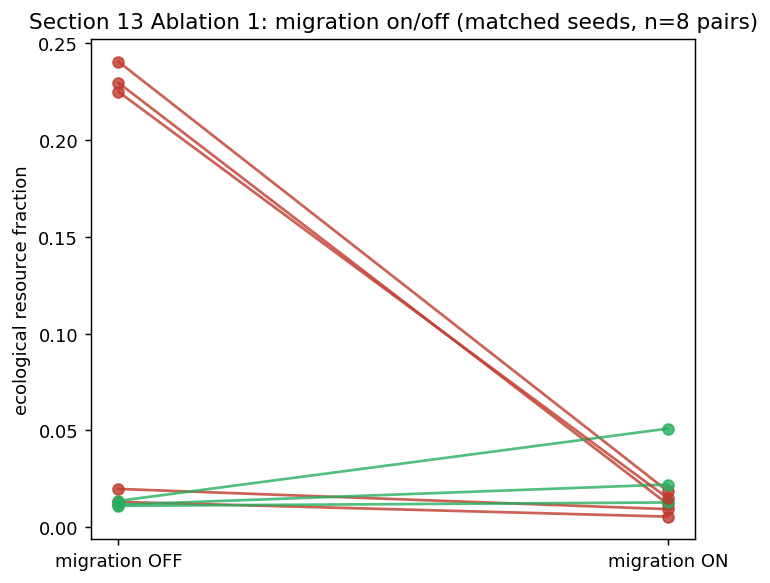
\includegraphics[width=0.85\textwidth]{figures/appendix/a_l12_stage13_migration_ablation.png}
\caption{Level 1.2 Section 13 matched-seed migration ablation
($n$=8 pairs): 5/8 pairs favor migration off on ecological fraction.}
\end{figure}

\begin{figure}[htbp]
\centering
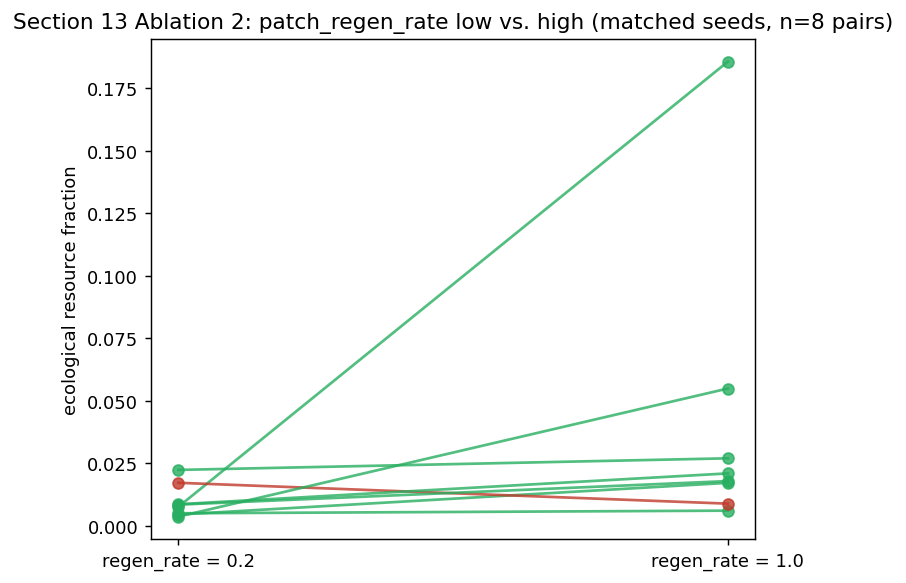
\includegraphics[width=0.85\textwidth]{figures/appendix/a_l12_stage13_regen_ablation.png}
\caption{Level 1.2 Section 13 matched-seed regeneration-rate ablation
($n$=8 pairs): 7/8 pairs favor the higher regeneration rate.}
\end{figure}

\begin{figure}[htbp]
\centering
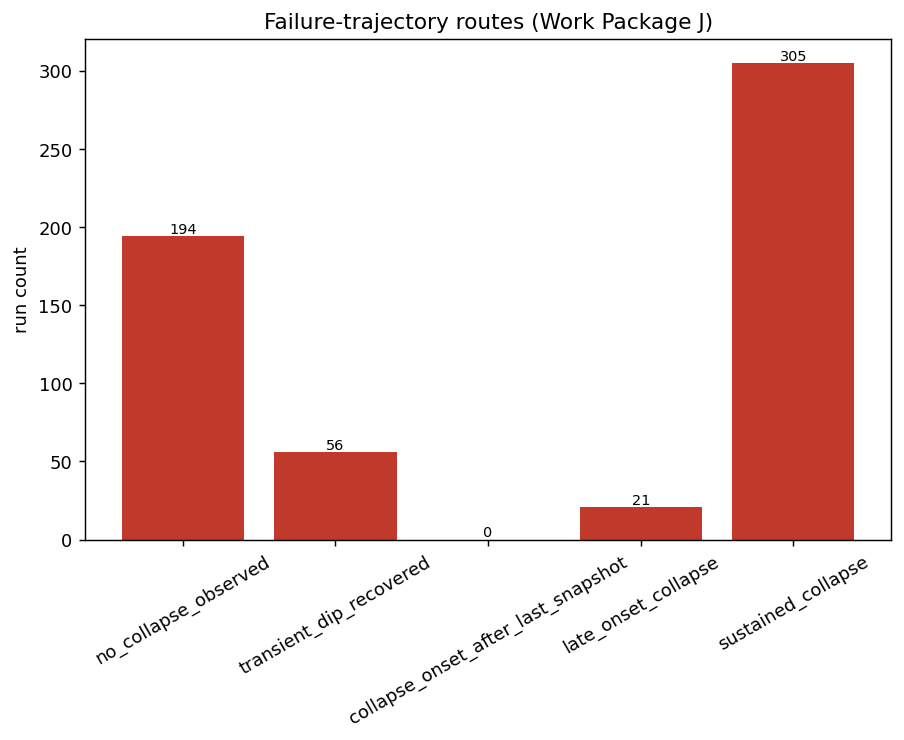
\includegraphics[width=0.75\textwidth]{figures/appendix/a_l12b_failure_trajectory.png}
\caption{Level 1.2b failure-trajectory classification, discovery pool
($n$=576): most collapse outcomes are \texttt{sustained\_collapse}, not a
last-instant artifact.}
\end{figure}

\begin{figure}[htbp]
\centering
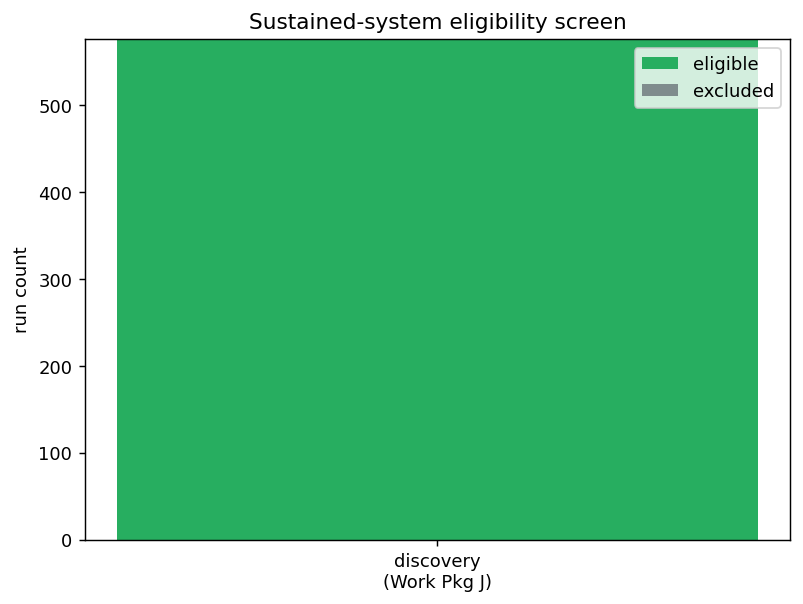
\includegraphics[width=0.7\textwidth]{figures/appendix/a_l12b_sustained_eligibility.png}
\caption{Level 1.2b sustained-system data-sufficiency screen: all 576
discovery runs eligible, 0 excluded, comfortably above both the preferred
(60) and hard-minimum (40) gates.}
\end{figure}

\begin{figure}[htbp]
\centering
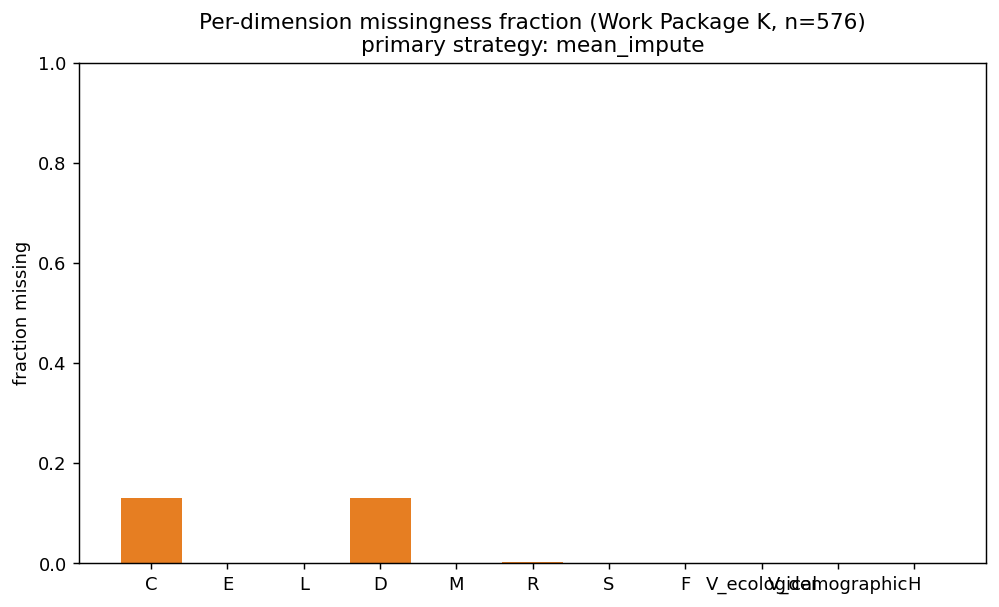
\includegraphics[width=0.7\textwidth]{figures/appendix/a_l12b_missingness.png}
\caption{Level 1.2b phenotype-feature missingness by dimension, discovery
pool ($n$=576).}
\end{figure}

\begin{figure}[htbp]
\centering
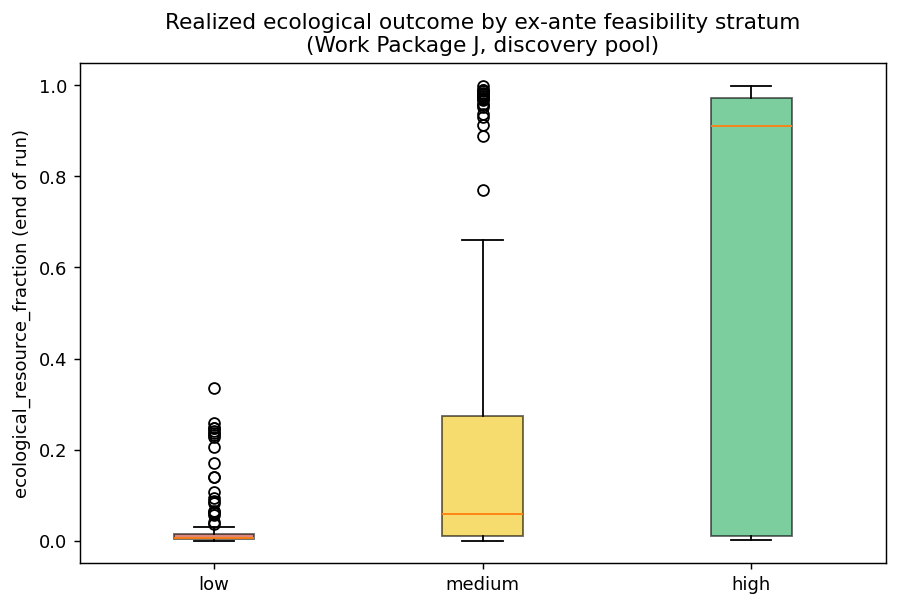
\includegraphics[width=0.85\textwidth]{figures/appendix/a_l12b_feature_by_stratum.png}
\caption{Level 1.2b phenotype-feature distributions by ecological stratum
(low/medium/high expected-pressure ratio).}
\end{figure}

\begin{figure}[htbp]
\centering
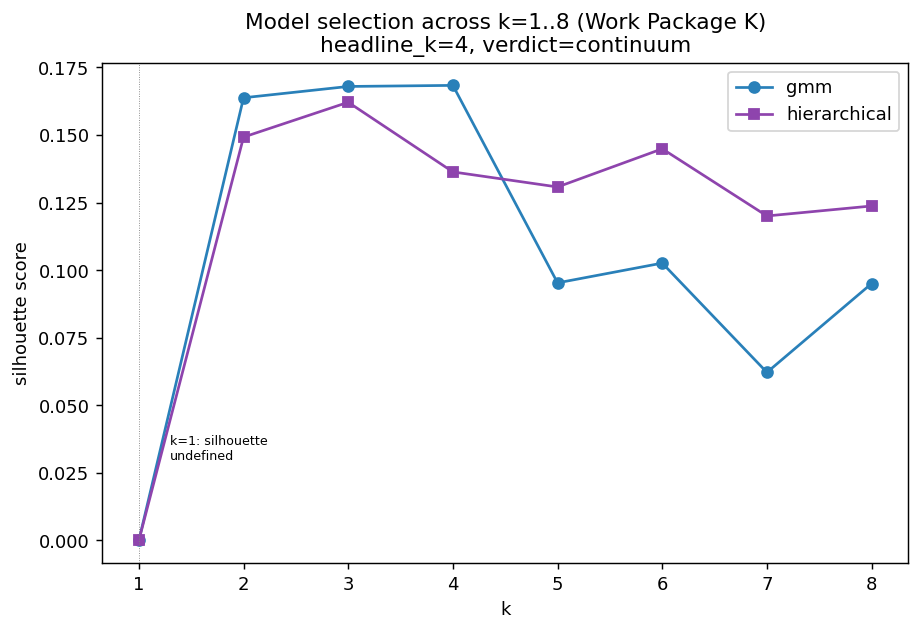
\includegraphics[width=0.8\textwidth]{figures/appendix/a_l12b_model_selection.png}
\caption{Level 1.2b model-selection metrics (silhouette,
Calinski--Harabasz, Davies--Bouldin) by $k$, discovery pool.}
\end{figure}

\begin{figure}[htbp]
\centering
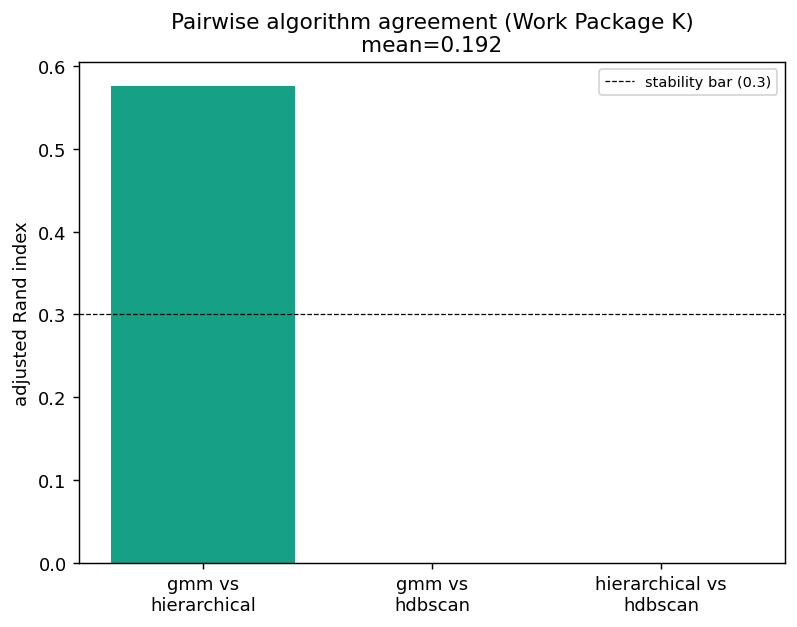
\includegraphics[width=0.75\textwidth]{figures/appendix/a_l12b_algorithm_agreement.png}
\caption{Level 1.2b pairwise algorithm-agreement (adjusted Rand index)
between Gaussian mixture, hierarchical, and \texttt{HDBSCAN} fits.}
\end{figure}

\begin{figure}[htbp]
\centering
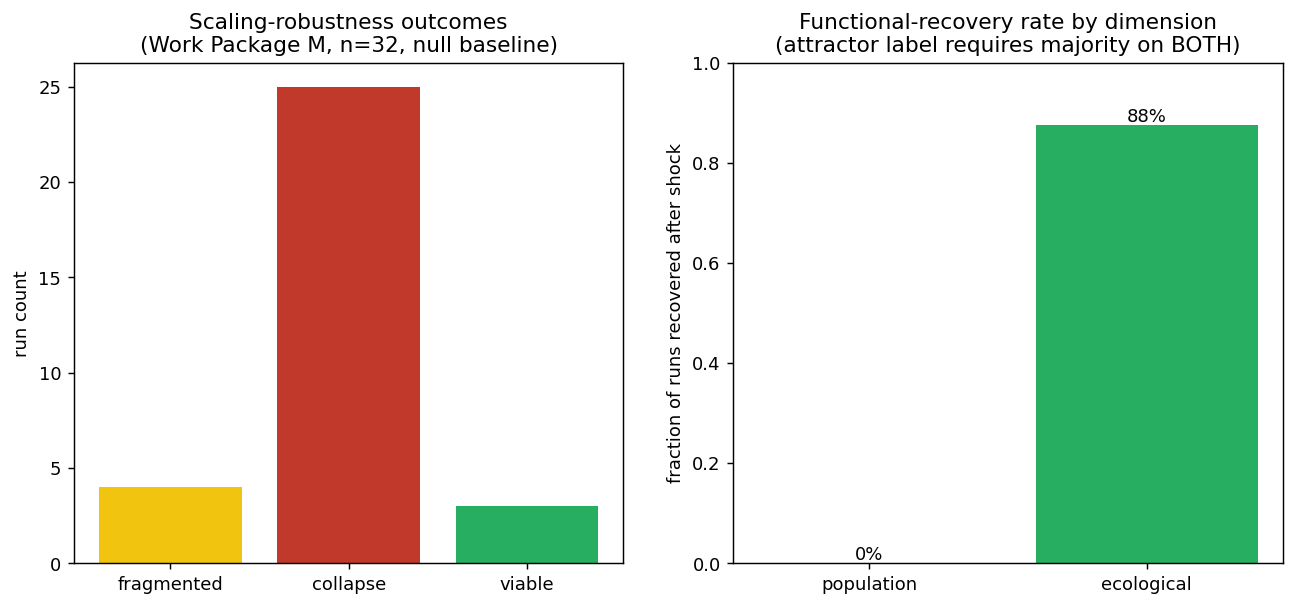
\includegraphics[width=0.85\textwidth]{figures/appendix/a_l12b_scaling_robustness.png}
\caption{Level 1.2b Work Package M scaling-robustness grid: outcome and
recovery detail across population $\times$ patch-count $\times$
modularity conditions ($n$=32).}
\end{figure}

\begin{figure}[htbp]
\centering
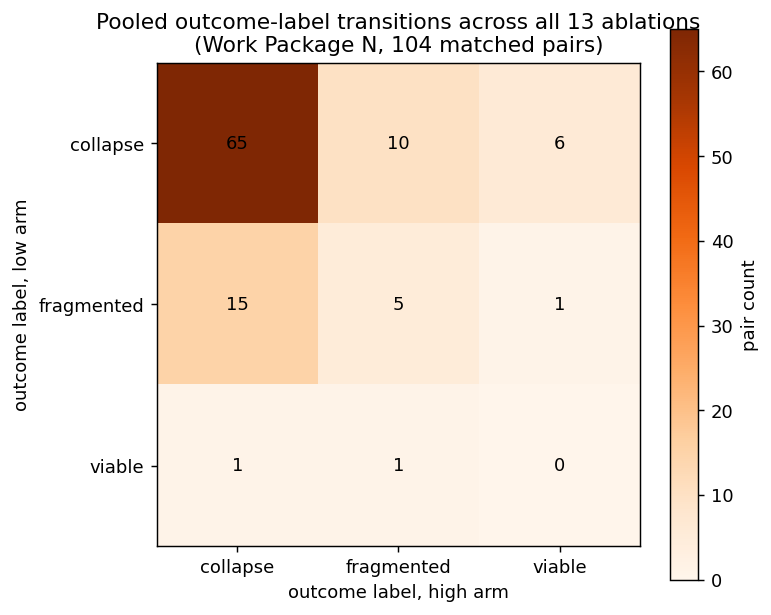
\includegraphics[width=0.75\textwidth]{figures/appendix/a_l12b_outcome_transition_matrix.png}
\caption{Level 1.2b outcome-label transition matrix, discovery versus
confirmation pools.}
\end{figure}

\begin{figure}[htbp]
\centering
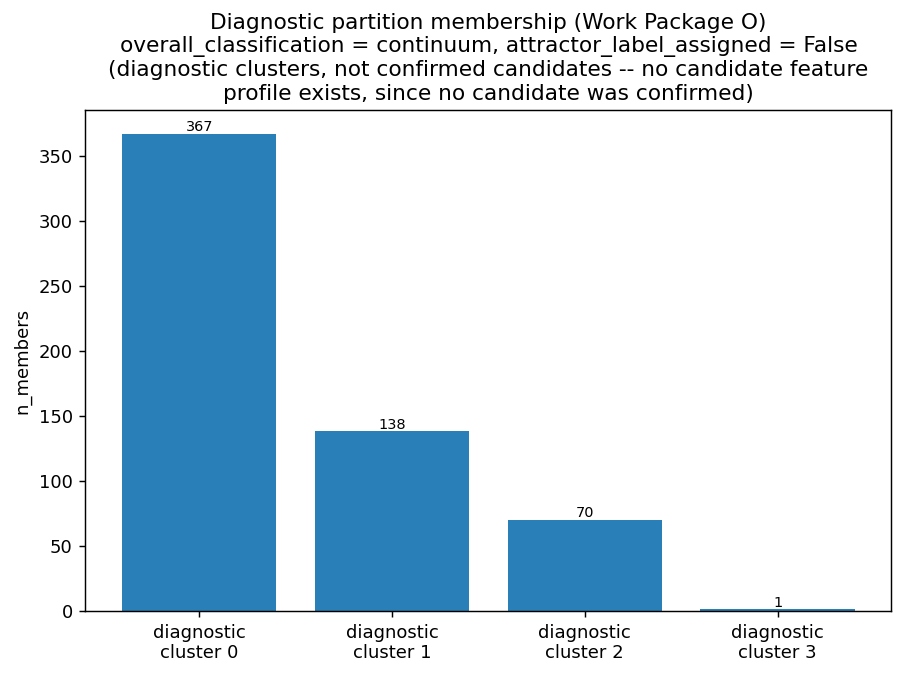
\includegraphics[width=0.75\textwidth]{figures/appendix/a_l12b_recurrence_classification.png}
\caption{Level 1.2b Work Package O overall recurrence classification
summary: \texttt{continuum}, \texttt{attractor\_label\_assigned=False}.}
\end{figure}

\begin{figure}[htbp]
\centering
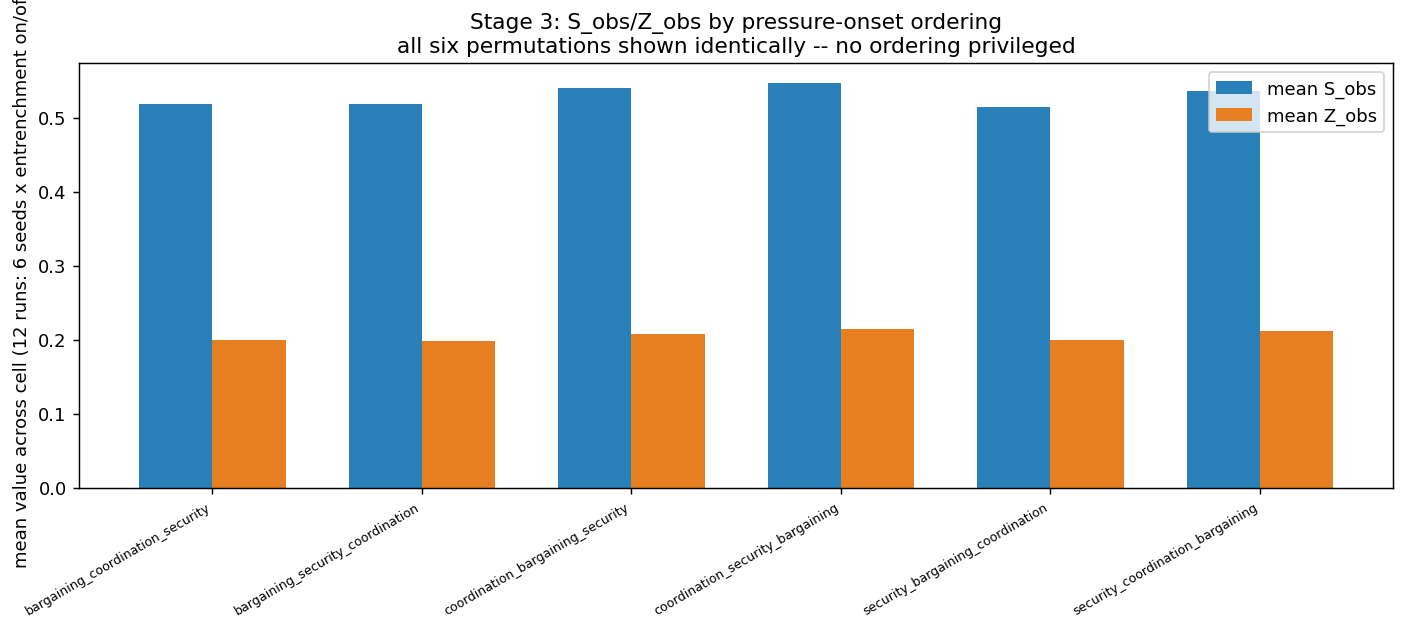
\includegraphics[width=0.85\textwidth]{figures/appendix/a_l13_stage3_by_ordering.png}
\caption{Level 1.3 Stage 3: mean $S_{\text{obs}}$/$Z_{\text{obs}}$ by
pressure-onset ordering (72-run matched factorial, six orderings),
descriptive precursor to Level 1.3b's own purpose-designed Stage 3
factorial (\cref{fig:l13b-ordering}).}
\end{figure}

\begin{figure}[htbp]
\centering
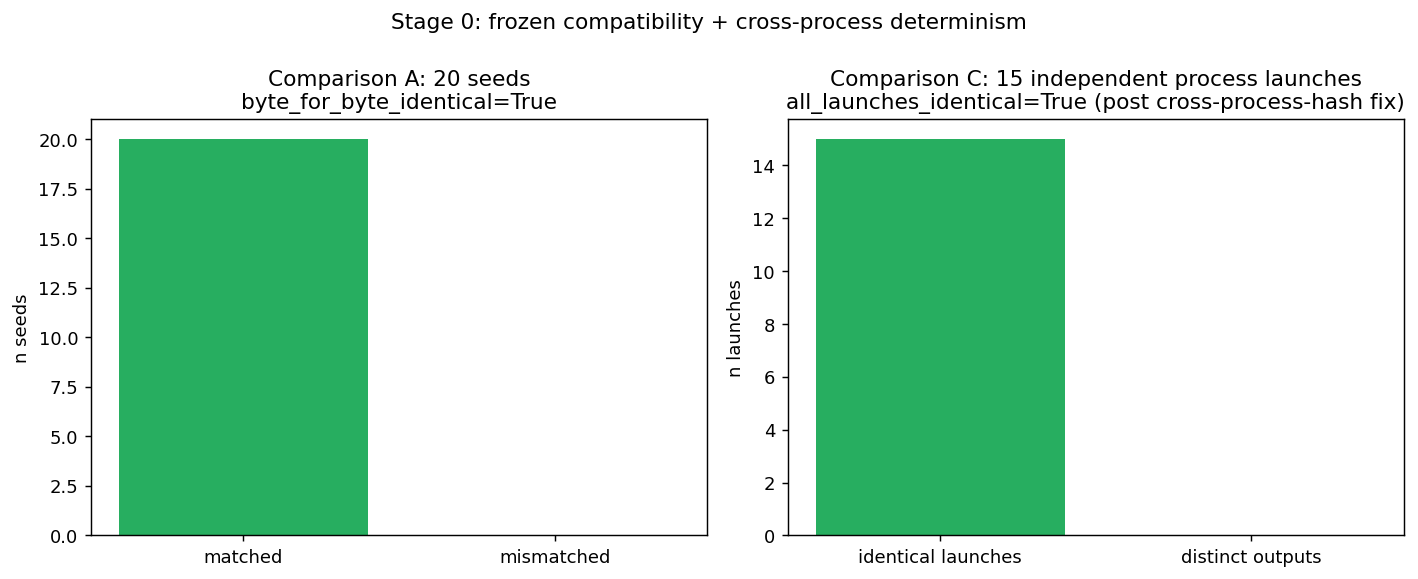
\includegraphics[width=0.75\textwidth]{figures/appendix/a_l13b_cross_process_repro.png}
\caption{Level 1.3b Stage 0: cross-process determinism comparison. 15
distinct outputs pre-fix (frozenset-hash non-determinism), 1 identical
output post-fix, across 15 separate process launches of the identical
seed and configuration.}
\end{figure}

\begin{figure}[htbp]
\centering
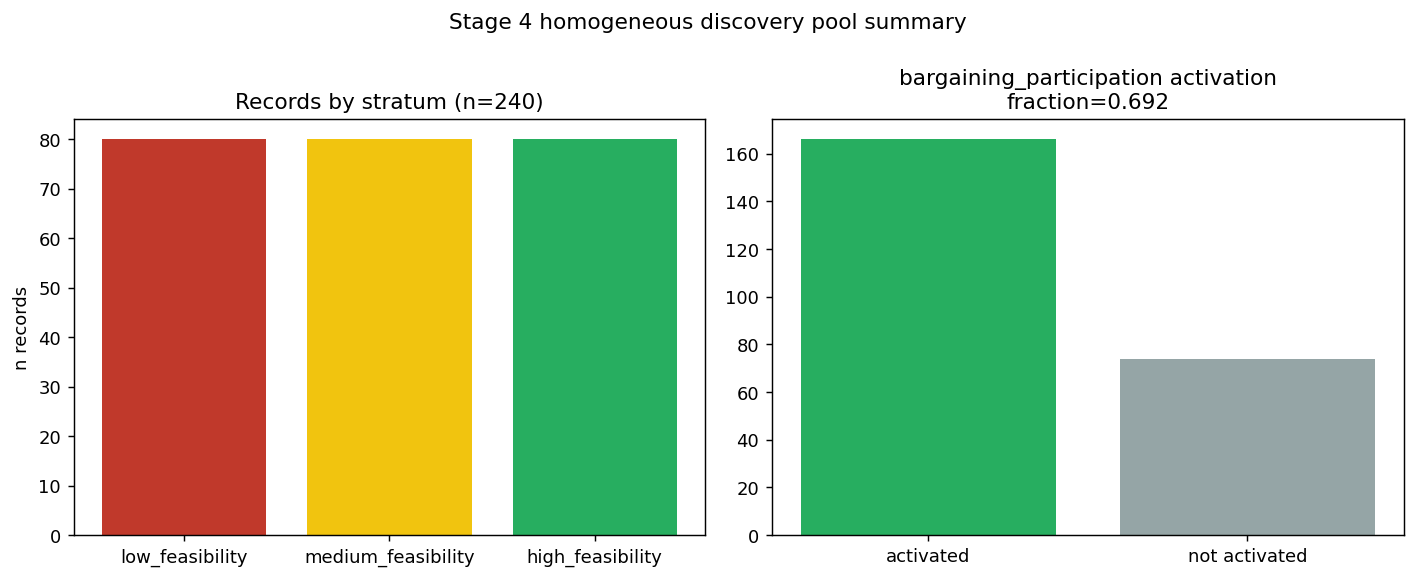
\includegraphics[width=0.8\textwidth]{figures/appendix/a_l13b_stage4_pool_summary.png}
\caption{Level 1.3b Stage 4: 240-run homogeneous discovery pool summary
(the purpose-designed successor to Level 1.3's own pooled 216-run
sample).}
\end{figure}

\begin{figure}[htbp]
\centering
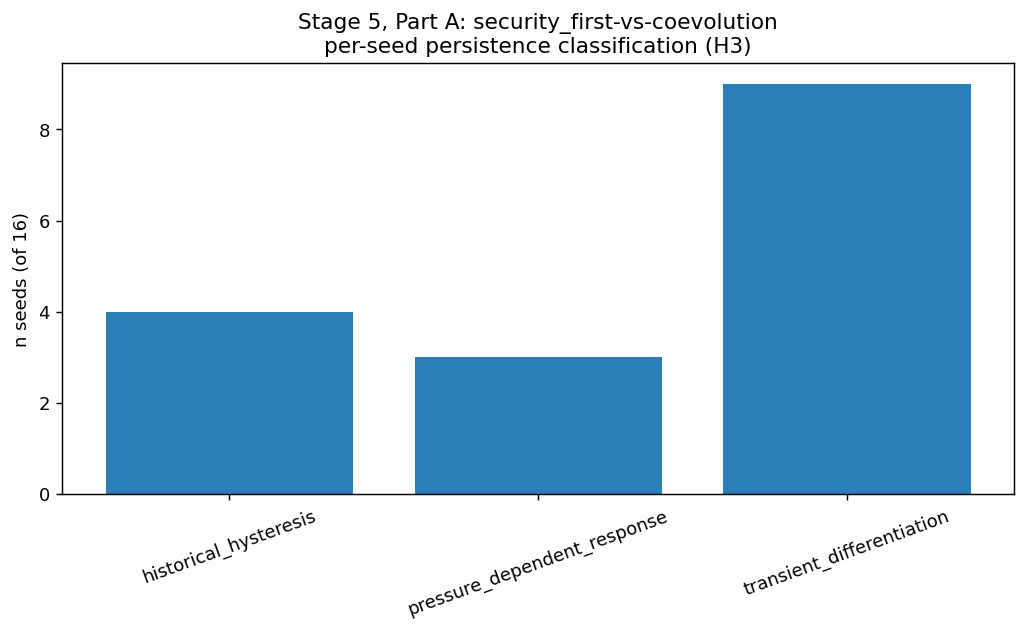
\includegraphics[width=0.8\textwidth]{figures/appendix/a_l13b_persistence_classification.png}
\caption{Level 1.3b Stage 5 Part A: per-seed persistence classification
(16 matched seeds, \texttt{security\_first} vs.\ \texttt{coevolution}) ---
9/16 \texttt{transient\_differentiation}, 4/16 \texttt{historical\_%
hysteresis}, 3/16 \texttt{pressure\_dependent\_response}, 0/16
\texttt{entrenched\_path\_dependence}.}
\end{figure}

\begin{figure}[htbp]
\centering
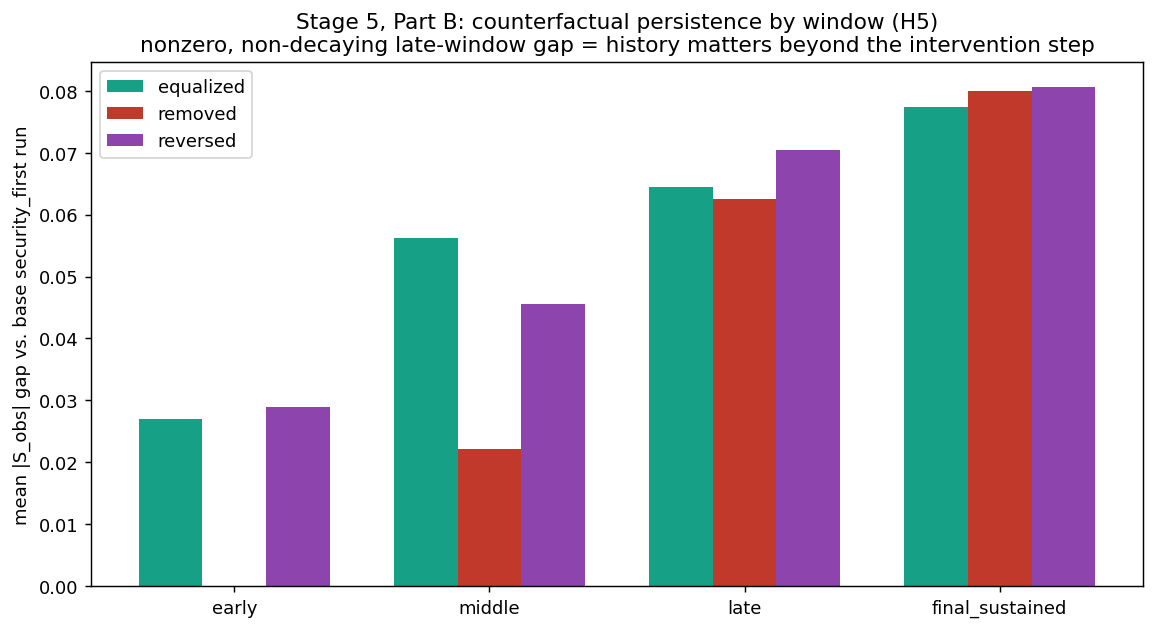
\includegraphics[width=0.8\textwidth]{figures/appendix/a_l13b_counterfactual_persistence.png}
\caption{Level 1.3b Stage 5 Part B: counterfactual-persistence gap by
window for the \texttt{removed}/\texttt{reversed}/\texttt{equalized}
pressure-history transforms versus the base \texttt{security\_first} run.}
\end{figure}

\begin{figure}[htbp]
\centering
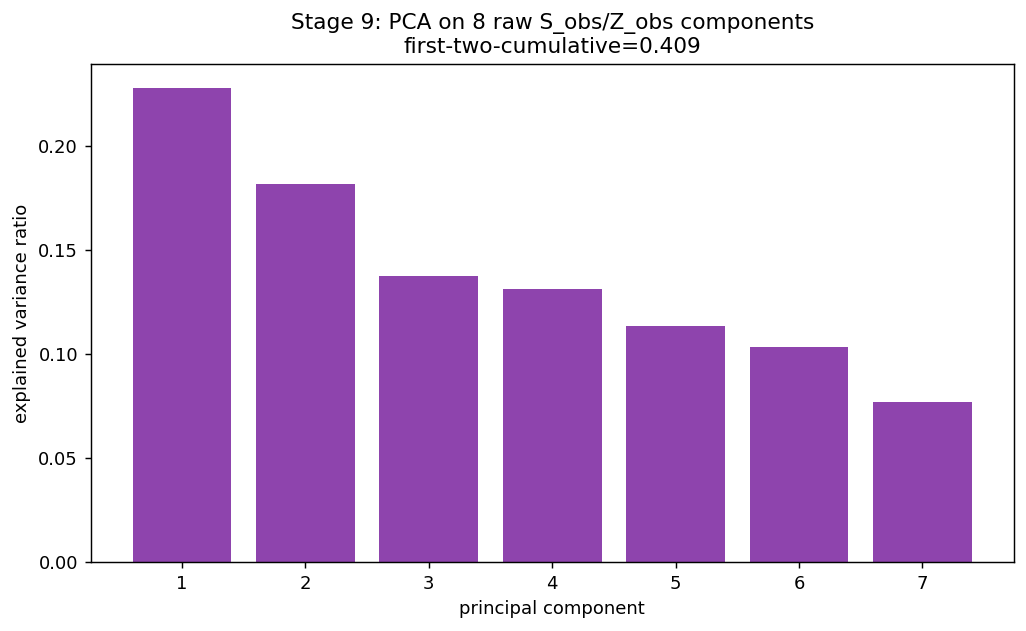
\includegraphics[width=0.75\textwidth]{figures/appendix/a_l13b_factor_structure.png}
\caption{Level 1.3b Stage 9: data-driven factor-structure analysis. PC1
(22.8\% of variance) is loaded by both legitimacy channels together
(0.654 performance, 0.674 procedural) rather than splitting cleanly along
an $S$-axis/$Z$-axis line; scree flat, top-two cumulative 40.9\%.}
\end{figure}

\begin{figure}[htbp]
\centering
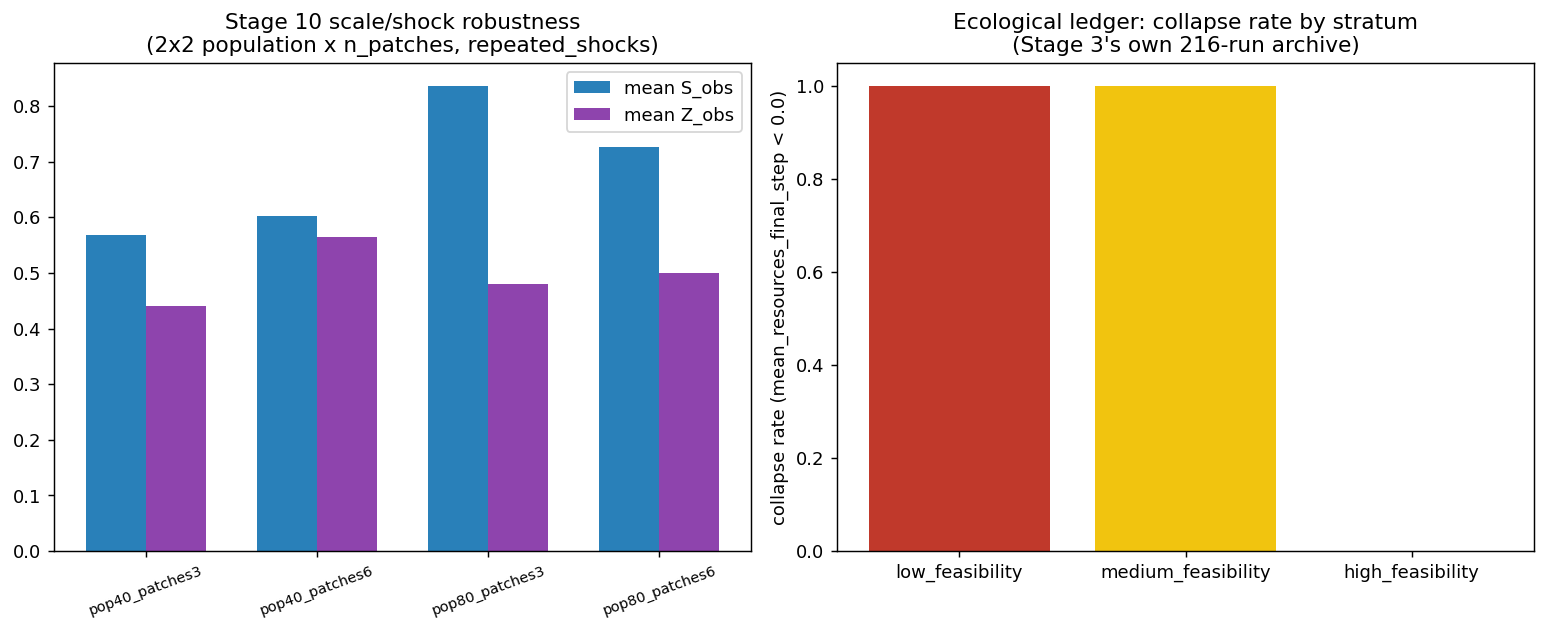
\includegraphics[width=0.75\textwidth]{figures/appendix/a_l13b_scale_and_ledger.png}
\caption{Level 1.3b Stage 10: ecological-control scale-shock check (24
runs) under the historically extended substrate.}
\end{figure}

\begin{figure}[htbp]
\centering
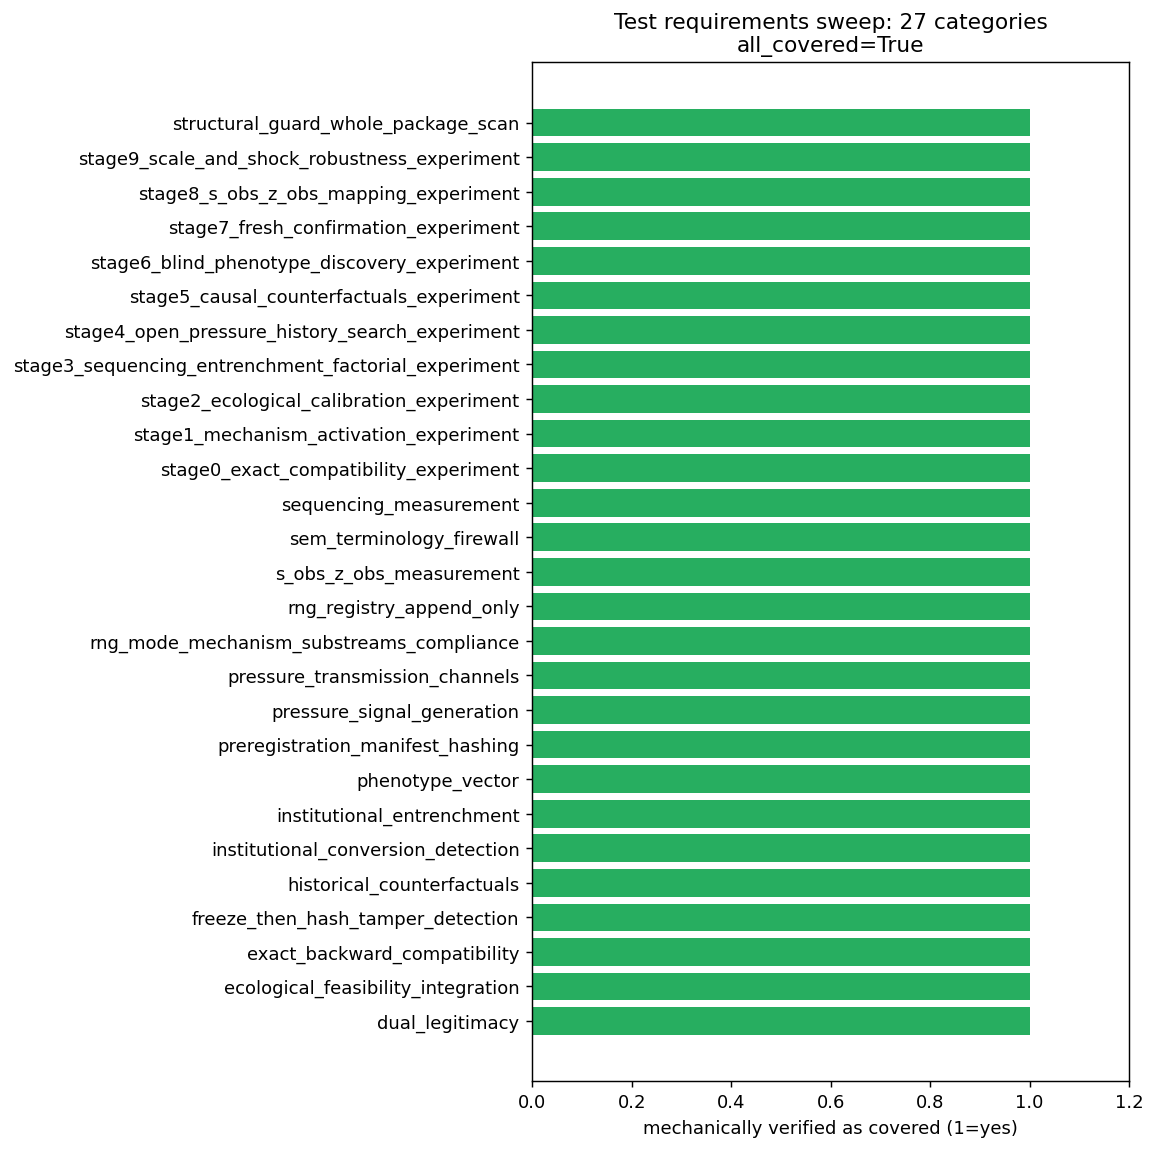
\includegraphics[width=0.9\textwidth]{figures/appendix/a_l13_test_requirements_coverage.png}
\caption{Level 1.3 test-requirements coverage matrix.}
\end{figure}

\begin{figure}[htbp]
\centering
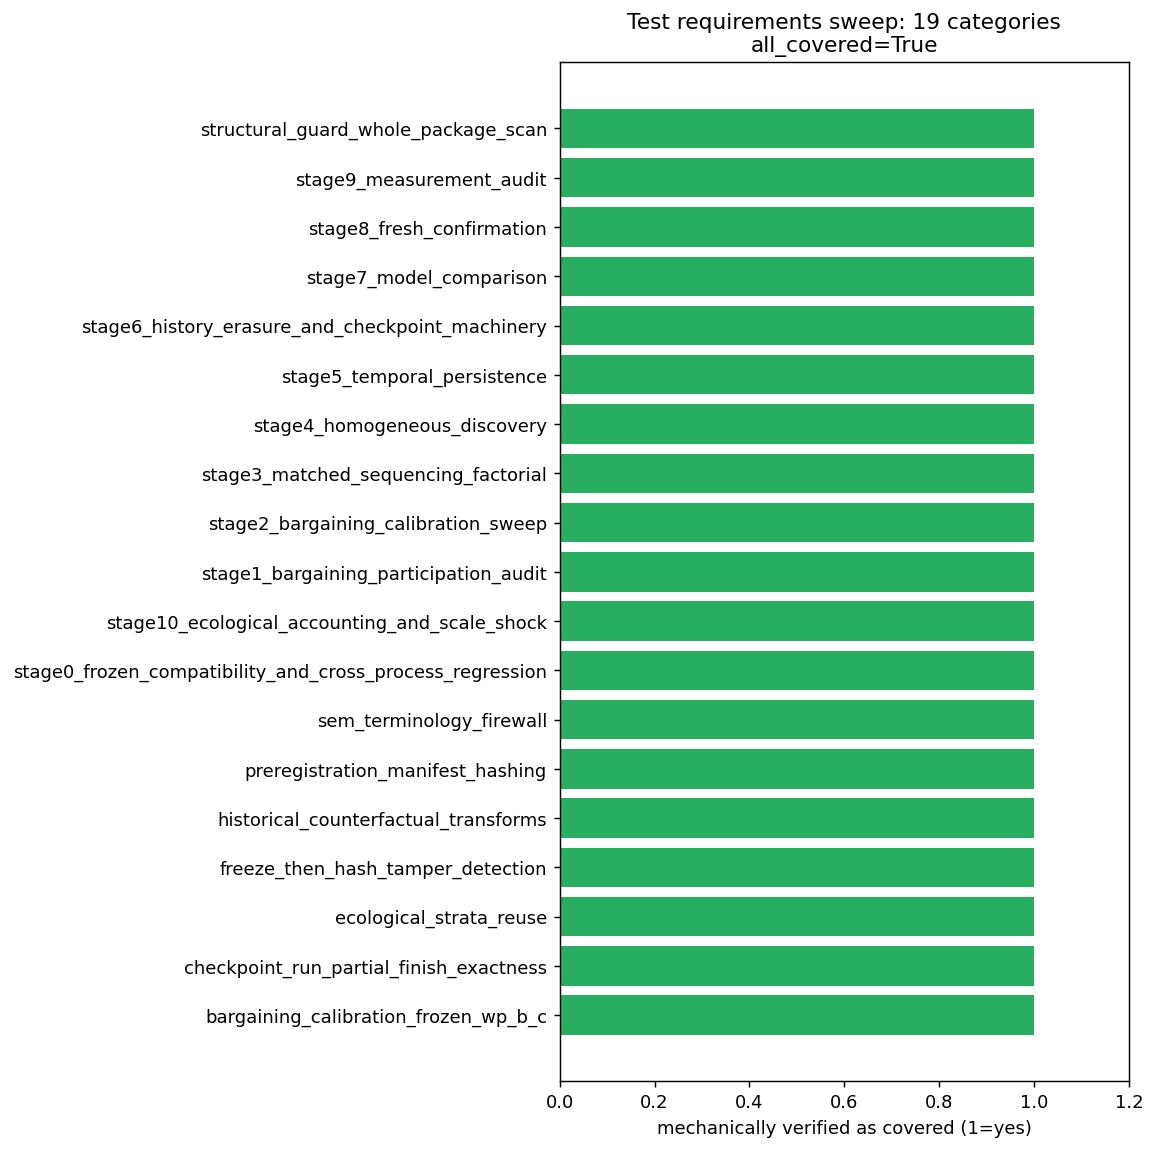
\includegraphics[width=0.9\textwidth]{figures/appendix/a_l13b_test_requirements_coverage.png}
\caption{Level 1.3b test-requirements coverage matrix (19 categories,
including two negative controls proving the checker can actually fail).}
\end{figure}
